\documentclass[a4paper,14pt]{extreport} % формат документа

\usepackage{amsmath}
\usepackage{cmap} % поиск в ПДФ
\usepackage[T2A]{fontenc} % кодировка
\usepackage[utf8]{inputenc} % кодировка исходного текста
\usepackage[english,russian]{babel} % локализация и переносы
\usepackage[left = 2cm, right = 1cm, top = 2cm, bottom = 2 cm]{geometry} % поля
\usepackage{listings}
\usepackage{graphicx} % для вставки рисунков
\usepackage{amsmath}
\usepackage{float}
\usepackage{multirow}
\graphicspath{{img/}}
\DeclareGraphicsExtensions{.pdf,.png,.jpg}
\newcommand{\anonsection}[1]{\section*{#1}\addcontentsline{toc}{section}{#1}}

\lstset{ %
	language=Lisp,                % Язык программирования 
	numbers=left,                   % С какой стороны нумеровать          
	frame=single,                    % Добавить рамку
}

\begin{document}
\begin{titlepage}

    \begin{table}[H]
        \centering
        \footnotesize
        \begin{tabular}{cc}
            \multirow{8}{*}{
\includegraphics[scale=0.35]{bmstu.jpg}}
            & \\
            & \\
            & \textbf{Министерство науки и высшего образования Российской Федерации} \\
            & \textbf{Федеральное государственное бюджетное образовательное учреждение} \\
            & \textbf{высшего образования} \\
            & \textbf{<<Московский государственный технический} \\
            & \textbf{университет имени Н.Э. Баумана>>} \\
            & \textbf{(МГТУ им. Н.Э. Баумана)} \\
        \end{tabular}
    \end{table}

    \vspace{-2.5cm}

    \begin{flushleft}
        \rule[-1cm]{\textwidth}{3pt}
        \rule{\textwidth}{1pt}
    \end{flushleft}

    \begin{flushleft}
        \small
        ФАКУЛЬТЕТ
        \underline{<<Информатика и системы управления>>\ \ \ \ \ \ \ 
        \ \ \ \ \ \ \ \ \ \ \ \ \ \ \ \ \ \ \ \ \ \ \ \ \ \ \ \ \ \ \ 
    \ \ \ \ \ \ \ \ \ \ \ \ \ \ \ } \\
        КАФЕДРА
        \underline{<<Программное обеспечение ЭВМ и
        информационные технологии>>
        \ \ \ \ \ \ \ \ \ \ \ \ \ \ \ \ \ \ \ \ }
    \end{flushleft}

    \vspace{2cm}

    \begin{center}
        \textbf{Лабораторная работа № 5} \\
        \vspace{0.5cm}
    \end{center}

    \vspace{4cm}

    \begin{flushleft}
        \begin{tabular}{ll}
            \textbf{Дисциплина} & Экономика программной инженерии.  \\
            \textbf{Тема} & Контроль хода выполнения проекта \\ 
            & с помощью средств анализа затрат. \\
            & Анализ рисков по методу PERT. Работа с отчетами. \\
            \\
            \textbf{Студент} & Сусликов Д.В. \\
            \textbf{Группа} & ИУ7-85Б \\
            \textbf{Оценка (баллы)} & \\
            \textbf{Преподаватель} & Барышникова М.Ю., Силантьева А.В.   \\
        \end{tabular}
    \end{flushleft}

    \vspace{4cm}

   \begin{center}
        Москва, 2022 г.
    \end{center}

\end{titlepage}

\begin{enumerate}

\item \textbf{Основное задание}

Содержание проекта: Команда разработчиков из 16 человек занимается созданием карты города на основе собственного модуля отображения. Проект должен быть завершен в течение 6 месяцев. Бюджет проекта: 50 000 рублей.

\item \textbf{Задание 1}

Выведем таблицу освоенного объема.

\begin{figure}[H]
  \centering
  \caption{Освоенный объем. }
  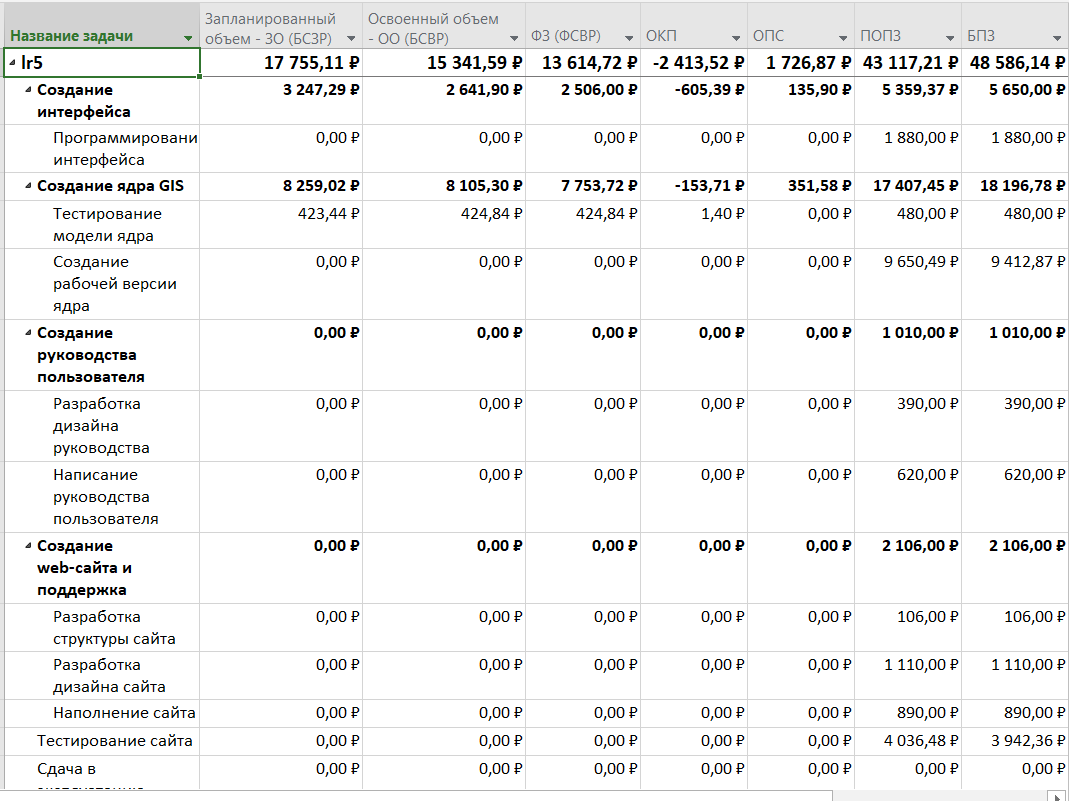
\includegraphics[scale=0.7]{11}
\end{figure}

Проанализируем затраты по методике освоенного объема:

\textbf{Запланированный объем (ЗО)} -- средства, которые были бы затрачены на выполнение задачи в период с начала проекта до выбранной даты отчета, если бы задача точно соответствовала графику и смете. В нашем проекте: 17755,11 рублей.

\textbf{Базовая стоимость выполненных работ (БСВР)}-- средства, которые были бы затрачены на выполнение задачи с самого начала проекта до выбранной даты отчета, если бы фактически выполненная работа оплачивалась согласно смете. В нашем проекте: 15341,59 рублей (отклонение от базовой стоимости запланированных работ - 2413,52 рублей).

\newpage
\textbf{Фактические затраты или фактическая стоимость выполненных работ (ФСВР)}-- средства, фактически потраченные на выполнение задачи в период с начала проекта до выбранной даты отчета. В случае проекта: 13614,72 рублей (отклонение от базовой стоимости выполненных работ -513,13 рублей). 

\textbf{Предварительная оценка по завершении (ПОПЗ)} -- ожидаемые общие затраты для задачи, расчет которых основан на предположении, что оставшаяся часть работы будет выполнена в точном соответствии со сметой. Для проекта: 43117.49 рублей.

\item \textbf{Задание 2}

Отобразим отчеты о бюджетной стоимости во вкладке <<Отчеты>> <<Наглядные отчеты>>.

\begin{figure}[H]
  \centering
  \caption{Отчет о бюджетной стоимости. }
  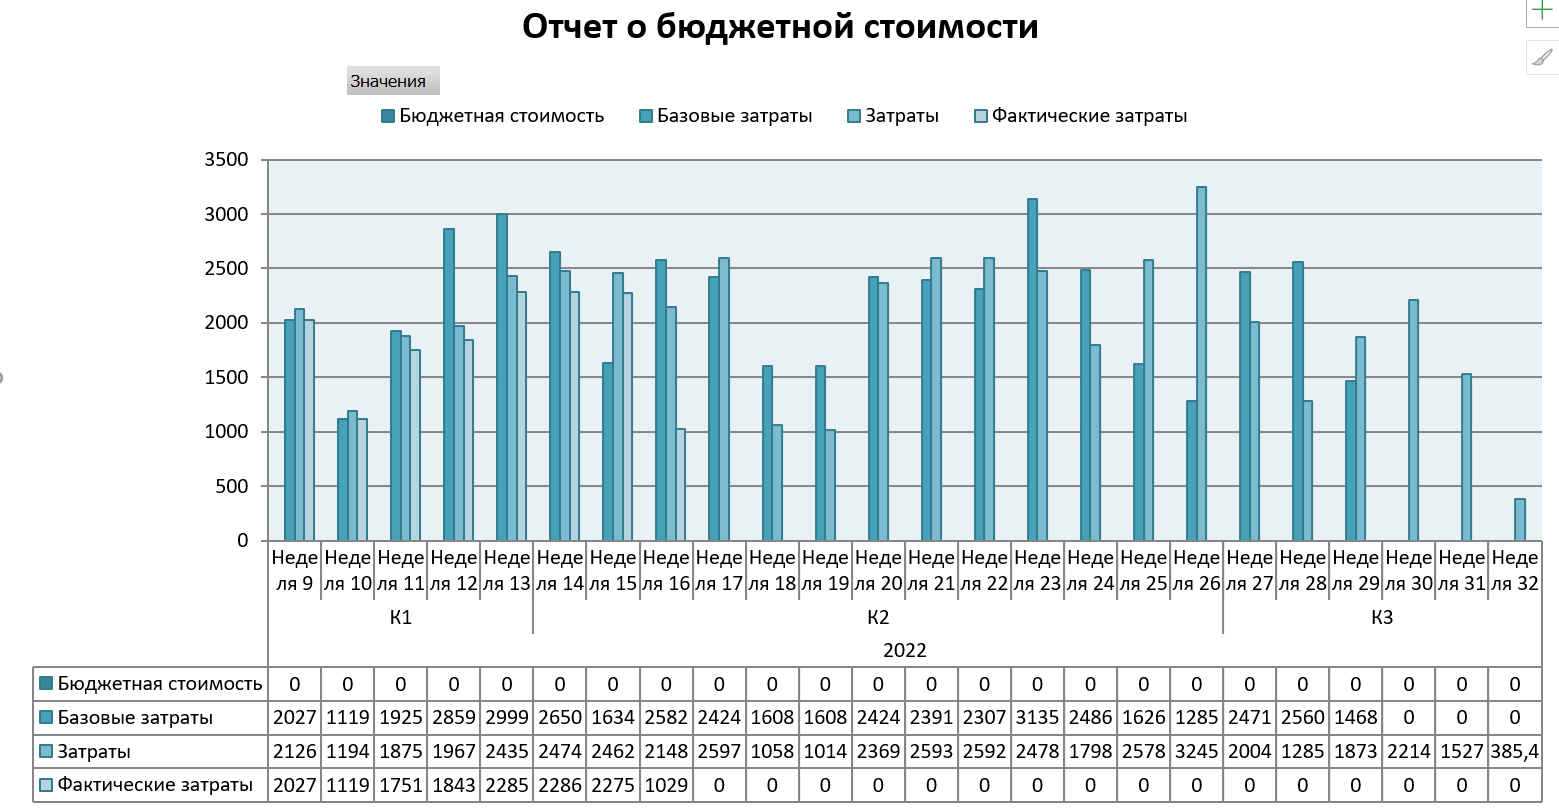
\includegraphics[scale=0.55]{22}
\end{figure}

Из приведенного графика следует, что наибольшие затраты пришлись на 26 неделю (27.06-1.07). 
В это время выполнялись задачи: программирование интерфейса, наполнение базы объектов, создание рабочей версии ядра, разработка дизайна руководства, написание руководства пользователя, разработка дизайна сайта.

Выведем на экран задачи, превышающие бюджетную стоимость.

\begin{figure}[H]
  \centering
  \caption{Превышение затрат. }
  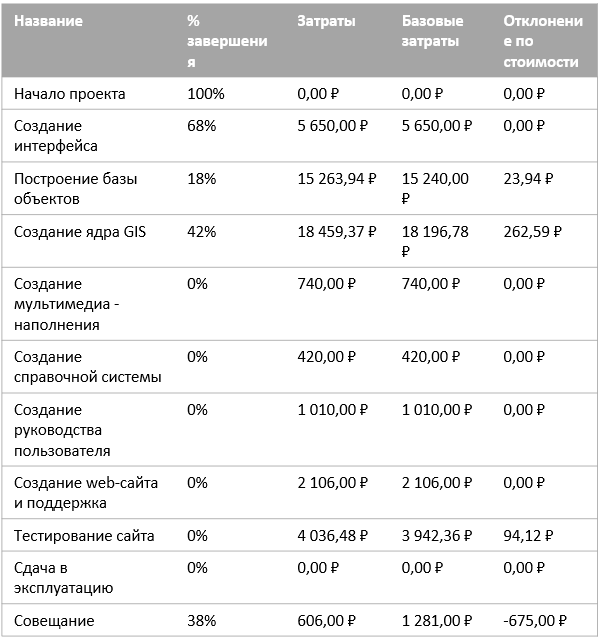
\includegraphics[scale=1]{33}
\end{figure}

Задачи построение базы объектов, создание ядра GIS, тестирование сайта превышают базовые затраты, однако удалось сократить расходы на совещаниях.

\item \textbf{Задание 3}

Предложим альтернативную декомпозицию работ по этапам разработки ПО.

 \begin{figure}[H]
  \centering
  \caption{Альтернативная декомпозиция. }
  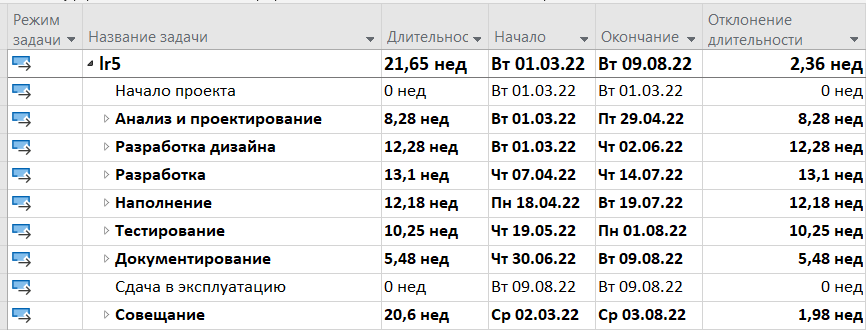
\includegraphics[scale=0.8]{44}
\end{figure}

В результате дата окончание не изменилась, а бюджет уменьшились до 48014 рублей, что сэкономило 572,14 рублей.
 \begin{figure}[H]
	\centering
	\caption{Альтернативная декомпозиция. }
	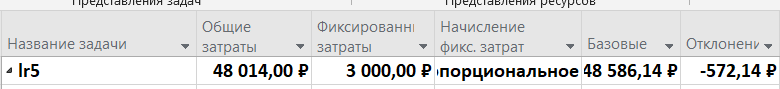
\includegraphics[scale=0.8]{442}
\end{figure}

\item \textbf{Вывод}

В проекте был проведен анализ базового и фактического плана на 20 апреля.

У руководителя проекта наибольшая потребность в средствах возникнет на 26 неделе. 

Проведен альтернативный вариант декомпозиции задачи, который оказался чуть лучше изначального (время окончания проекта не изменилось, однако бюджет уменьшился на 572,14 рублей), так что лучшим вариантом будет оставить альтернативный вариант.

\end{enumerate}

\end{document}